\documentclass{article}
\usepackage[utf8]{inputenc}
\usepackage{amsmath}
\usepackage{listings}
\usepackage{tikz}
\usepackage[backend=biber,style=numeric]{biblatex}
\addbibresource{references.bib}
\usetikzlibrary{trees}
\usetikzlibrary{arrows.meta}
\title{The Mechanics of Red-Black Trees: A Visual Approach}
\author{Antonios Kordatzakis}
\date{\today}

\newcommand\encircle[1]{%
  \tikz[baseline=(X.base)] 
    \node (X) [draw, shape=circle, minimum size=14, inner sep=0, font=\small] {\strut #1};}

\begin{document}
\maketitle

\section{Introduction}

A \emph{Red-Black} tree \cite{bayer, guibas} is a self-balancing binary search tree in which every \emph{link}
carries an additional \emph{COLOR} attribute, taking the value \emph{RED} or \emph{BLACK}.
This attribute serves to prevent the tree from becoming unbalanced.
It should be noted that the \emph{COLOR} attribute belongs to a \emph{link} rather than to a \emph{node} of the tree.
As will be shown, when the \emph{Red-Black} tree is modeled in the algorithms and the implementation,
the absence of a class representing a \emph{link} leads us to store the \emph{COLOR} property in the tree node class.
Accordingly, when a node is described as \emph{RED} or \emph{BLACK},
the intended meaning is that the link from its parent to that node is \emph{RED} or \emph{BLACK}.

\par
The operations of a \emph{Red-Black} tree are more readily understood when the tree is visualized as in
\cite{bayer}, that is, as a tree in which:

\begin{itemize}
    \item a \emph{RED} link connects two nodes at the same level.
    \item a \emph{BLACK} link increases the level by one.
\end{itemize}

Since the objective is to construct a balanced tree, two consecutive \emph{RED} links are not permitted. A single
\emph{left RED} link and a single \emph{right RED} link may originate from the same node, but the following link must be
\emph{BLACK}. For convenience, and to simplify the algorithms used to manipulate a \emph{Red-Black} tree,
the color of the root of the tree is set to \emph{BLACK}, although an implementation may choose to disregard this
convention.

In \cite{llrb, sedgewick} all \emph{RED} nodes lean to the left. The present work adopts the original definition of
\emph{Red-Black} trees, which admits both left and right \emph{RED} nodes.

\par
Consider a \emph{Red-Black} tree into which the following keys have been inserted: 11, 2, 14, 1, 7, 15, 5 and 8.
The resulting tree, whose root node has key \emph{11}, is shown in Figure~\ref{fig:red_black_tree}.

\begin{figure}[ht]
\centering
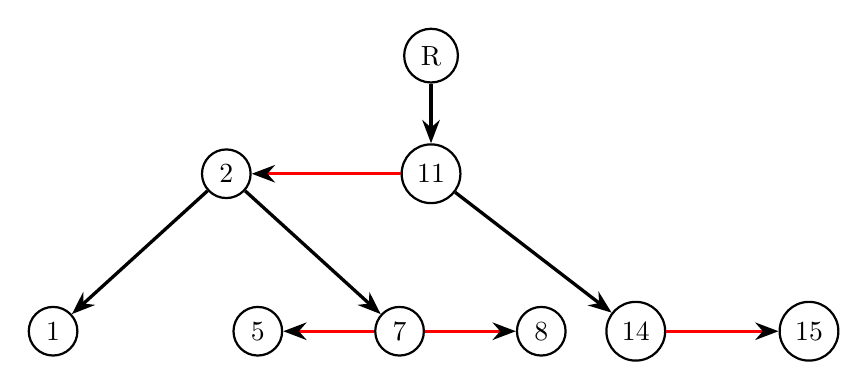
\begin{tikzpicture}
\begin{scope}[every node/.style={circle,thick,draw}]
    \node (Root) at (0.00, 1.50) {R};
    \node (11) at (0.00, 0.00) {11};
    \node (2) at (-2.60, 0.00) {2};
    \node (1) at (-4.80, -2.00) {1};
    \node (7) at (-0.40, -2.00) {7};
    \node (5) at (-2.20, -2.00) {5};
    \node (8) at (1.40, -2.00) {8};
    \node (14) at (2.60, -2.00) {14};
    \node (15) at (4.80, -2.00) {15};
\end{scope}
\begin{scope}[>={Stealth[black]},
              every node/.style={fill=white,circle},
              red_edge/.style={draw=red,very thick},
              black_edge/.style={draw=black,very thick}]
    \path [->] (Root) edge [black_edge] ({11});
    \path [->] (11) edge [red_edge] ({2});
    \path [->] (2) edge [black_edge] ({1});
    \path [->] (2) edge [black_edge] ({7});
    \path [->] (7) edge [red_edge] ({5});
    \path [->] (7) edge [red_edge] ({8});
    \path [->] (11) edge [black_edge] ({14});
    \path [->] (14) edge [red_edge] ({15});
\end{scope}
\end{tikzpicture}
\caption{A Red-Black tree}
\label{fig:red_black_tree}
\end{figure}

All \emph{leaf} nodes of the \emph{Red-Black} tree above lie at the same level; the tree is therefore balanced.

In general, the construction of a self-balancing tree requires two mechanisms:
\begin{itemize}
    \item a mechanism to propagate violations of balance to the level above,
    until no further violations remain --- the \emph{Propagation} mechanism.
    \item a mechanism to locally balance an unbalanced sub-tree --- the \emph{Rebalance} mechanism.
\end{itemize}

The \emph{COLOR} property is used to create these two mechanisms in \emph{Red-Black} trees.

\section{Properties of the Red-Black trees}
As noted above, for convenience the \emph{COLOR} is modeled as an attribute of the node rather than of the link.
The following rules apply to any \emph{Red-Black} tree:
\begin{enumerate}
   \item A node is either \emph{RED} or \emph{BLACK};
   that is, the link towards this node is either \emph{RED} or \emph{BLACK}.
   \item The \emph{root} is \emph{BLACK}.
   \item A \texttt{NIL} leaf is \emph{BLACK}.
   \item Both children of a \emph{RED} node should be \emph{BLACK}.
   \item Every simple path from \emph{root} to a leaf has the same number of \emph{BLACK} nodes.
\end{enumerate}

\section{Fixing violations}

When a new node is inserted into a \emph{Red-Black} tree, it is always connected to its parent by a \emph{RED} link.
A \emph{BLACK} link is not used, since it would alter the height of the tree, which is undesirable:
correcting a height violation caused by the insertion of a \emph{BLACK} node is a more difficult task than
correcting violations arising from \emph{RED} nodes.
Furthermore, the height of the tree is kept to a minimum for as long as no violation is present.
When there is no room for the new node and a new level must be introduced,
this is achieved by moving upwards and correcting any new violations that arise.
In every case---whether during an insertion, a deletion, or a correction---the height of the tree is,
where possible, kept unchanged.

No violation can occur when the parent of the new node is \emph{BLACK}:
\begin{itemize}
    \item no two consecutive \emph{RED} nodes are created, since the parent is \emph{BLACK}.
    \item the number of \emph{BLACK} nodes remains unchanged, since the new node is \emph{RED}.
\end{itemize}

It therefore suffices to examine the cases in which the parent of the new node is \emph{RED}.
To correct these violations, rotations such as those in \cite{clrs} are not used; instead, the visual representation of
the violation is allowed to guide the algorithms.

It should be borne in mind that, once a violation has been corrected, a new violation may arise at a higher level;
consequently the corrections may have to be applied to an ancestor of the current node, until a \emph{BLACK} link is
reached.

This section examines the three distinct types of violation that arise when working with \emph{Red-Black} trees.
Together with their three symmetrical counterparts, this yields a total of six distinct types of violation.

The term ``uncle'' of a node denotes the sibling of the node's parent
\footnote{Equivalently, the child of the grand-parent that is not the parent of the node.}.
The color of the uncle determines how the violation is corrected.

\subsection{Case 1: Red uncle --- Propagation mechanism}

Suppose we are given a \emph{Red-Black} tree with nodes
\encircle{11}, \encircle{2} and \encircle{14}, together with the parent of node \encircle{11}, denoted \encircle{p}
\footnote{The children of all nodes need not be shown, since the correction does not affect them.} 
; see Figure~\ref{fig:case_1_initial_tree}.

\begin{figure}[ht]
\centering
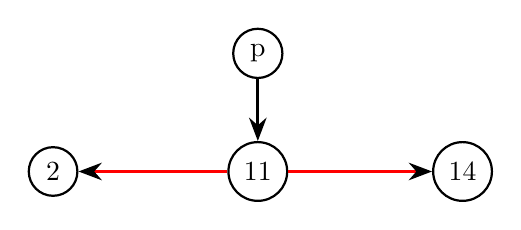
\begin{tikzpicture}
\begin{scope}[every node/.style={circle,thick,draw}]
    \node (p11) at (0.00, 1.50) {p};
    \node (11) at (0.00, 0.00) {11};
    \node (2) at (-2.60, 0.00) {2};
    \node (14) at (2.60, 0.00) {14};
\end{scope}
\begin{scope}[>={Stealth[black]},
              every node/.style={fill=white,circle},
              red_edge/.style={draw=red,very thick},
              black_edge/.style={draw=black,very thick}]
    \path [->] (p11) edge [black_edge] ({11});
    \path [->] (11) edge [red_edge] ({2});
    \path [->] (11) edge [red_edge] ({14});
\end{scope}
\end{tikzpicture}
\caption{The initial tree}
\label{fig:case_1_initial_tree}
\end{figure}

The link $p \rightarrow 11$ must be \emph{BLACK}; otherwise there would be two consecutive \emph{RED} links,
which is invalid.
If node \encircle{p} has height $h$, then node \encircle{11} has height $h+1$,
which is also the height of nodes \encircle{2} and \encircle{14}.

\begin{figure}[ht]
\centering
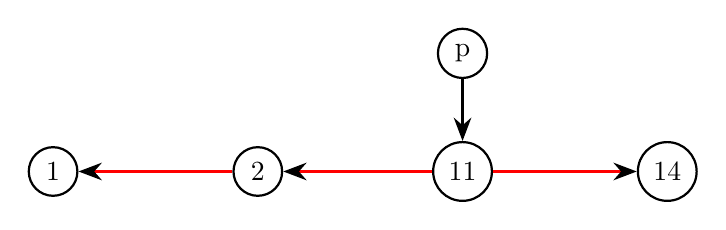
\begin{tikzpicture}
\begin{scope}[every node/.style={circle,thick,draw}]
    \node (p11) at (0.00, 1.50) {p};
    \node (11) at (0.00, 0.00) {11};
    \node (1) at (-5.20, 0.00) {1};
    \node (2) at (-2.60, 0.00) {2};
    \node (14) at (2.60, 0.00) {14};
\end{scope}
\begin{scope}[>={Stealth[black]},
              every node/.style={fill=white,circle},
              red_edge/.style={draw=red,very thick},
              black_edge/.style={draw=black,very thick}]
    \path [->] (p11) edge [black_edge] ({11});
    \path [->] (11) edge [red_edge] ({2});
    \path [->] (2) edge [red_edge] ({1});
    \path [->] (11) edge [red_edge] ({14});
\end{scope}
\end{tikzpicture}
\caption{Inserting a new node --- uncle is \emph{RED}}
\label{fig:case_1_violation}
\end{figure}


Consider now the insertion of node \encircle{1} shown in Figure~\ref{fig:case_1_violation}.
The two consecutive \emph{RED} links
$11 \rightarrow 2$ and $2 \rightarrow 1$ constitute a violation that must be corrected.
The uncle of node \encircle{1} is node \encircle{14}, which is \emph{RED}.
A new level is therefore introduced. In \emph{Red-Black} trees, levels are always created by moving upwards;
consequently node \encircle{11} is raised by one level.
As a result of introducing this level, the parent of node \encircle{11} has height $h$,
node \encircle{11} has height $h+1$, and nodes \encircle{2} and \encircle{14} have height $h+2$.
However, in order not to alter the level of the \emph{leaf} nodes,
the color of the link $p \rightarrow 11$ must be changed from \emph{BLACK} to \emph{RED},
which restores the heights of the nodes to their previous values (see Figure~\ref{fig:case_1_fix}).

\begin{figure}[ht]
\centering
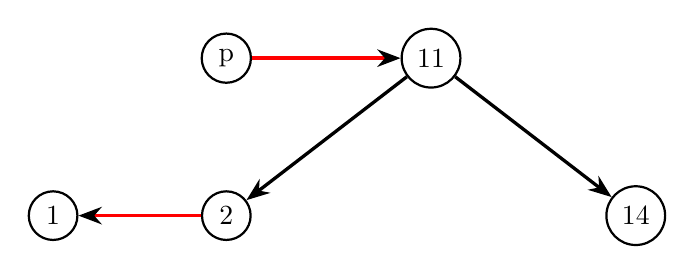
\begin{tikzpicture}
\begin{scope}[every node/.style={circle,thick,draw}]
    \node (p11) at (-2.60, 0.00) {p};
    \node (11) at (0.00, 0.00) {11};
    \node (2) at (-2.60, -2.00) {2};
    \node (1) at (-4.80, -2.00) {1};
    \node (14) at (2.60, -2.00) {14};
\end{scope}
\begin{scope}[>={Stealth[black]},
              every node/.style={fill=white,circle},
              red_edge/.style={draw=red,very thick},
              black_edge/.style={draw=black,very thick}]
    \path [->] (p11) edge [red_edge] ({11});
    \path [->] (11) edge [black_edge] ({2});
    \path [->] (2) edge [red_edge] ({1});
    \path [->] (11) edge [black_edge] ({14});
\end{scope}
\end{tikzpicture}
\caption{Fix of \emph{Case 1} violation}
\label{fig:case_1_fix}
\end{figure}

Because the color of the link $p \rightarrow 11$ has been changed from \emph{BLACK} to \emph{RED},
it is necessary to verify whether a new violation has been introduced.
Upon completion of this operation, 
the node under consideration becomes the grand-parent of the newly created node \encircle{11}.

If node \encircle{11} is the \emph{root} of the tree,
then the link $p \rightarrow 11$ must be changed back to \emph{BLACK}.

This correction realizes the \emph{Propagation} mechanism of \emph{Red-Black} trees:
it propagates the balance violation to the level above,
until a \emph{BLACK} link or the \emph{root} of the tree is reached.

\subsection{Case 2: Black uncle --- Rebalance mechanism}

Consider now the case in which the uncle of an invalid node is \emph{BLACK}.
Two cases arise, according to whether the new node is the \emph{left} or the \emph{right} child of its parent.

It should also be noted that both cases \emph{prepare} the ``uncle'' node for a subsequent \emph{Propagation}
by turning it into a \emph{RED} node.

\subsubsection{Case 2.1: Right child}

Suppose that keys have been inserted into a \emph{Red-Black} tree
and that the node under consideration is node \encircle{7},
which is the right child of its parent, node \encircle{1} Figure~\ref{fig:case_2_1_violation}.
The uncle of node \encircle{7} is node \encircle{14}, which is a \emph{BLACK} node.
Both cases implement the \emph{Rebalance} mechanism of \emph{Red-Black} trees.

\begin{figure}[ht]
\centering
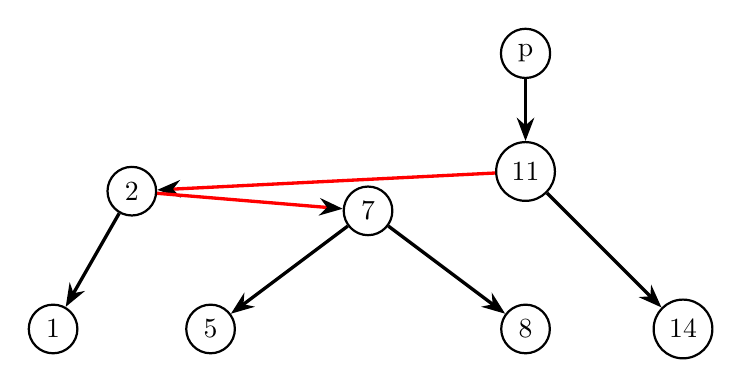
\begin{tikzpicture}
\begin{scope}[every node/.style={circle,thick,draw}]
    \node (p) at (0,1.5) {p};
    \node (11) at (0,0) {11};
    \node (2) at (-5,-0.25) {2};
    \node (14) at (2,-2) {14};
    \node (1) at (-6,-2) {1};
    \node (7) at (-2,-0.5) {7};
    \node (5) at (-4,-2) {5};
    \node (8) at (0,-2) {8};
\end{scope}
\begin{scope}[>={Stealth[black]},
              every node/.style={fill=white,circle},
              red_edge/.style={draw=red,very thick},
              black_edge/.style={draw=black,very thick}]
    \path [->] (p) edge [black_edge] (11);
    \path [->] (11) edge [red_edge] (2);
    \path [->] (2) edge [red_edge] (7);
    \path [->] (2) edge [black_edge] (1);
    \path [->] (11) edge [black_edge] (14);
    \path [->] (7) edge [black_edge] (8);
    \path [->] (7) edge [black_edge] (5);
\end{scope}
\end{tikzpicture}
\caption{Inserting a new node --- zig-zag, uncle is \emph{BLACK}}
\label{fig:case_2_1_violation}
\end{figure}

This is clearly not a valid \emph{Red-Black} tree, on account of the two consecutive \emph{RED} links
$11 \rightarrow 2$ and $2 \rightarrow 7$;
it may, however, be regarded as a temporary arrangement arising while other violations are being corrected as one moves
upwards, until a \emph{BLACK} link is reached.
It is readily seen that the tree ``leans'' to the left, a condition that requires correction.

Observe that node \encircle{7} naturally belongs between node \encircle{2} and node \encircle{11}. 
Since node \encircle{7} will connect node \encircle{2} and node \encircle{11}, its current children must be detached.
At the same time node \encircle{2} loses its right child and node \encircle{11} loses its left child.
In order to preserve the binary search tree property,
node \encircle{2} is connected to node \encircle{5} and node \encircle{11} to node \encircle{8}.

Accordingly, this violation is corrected as follows:
\begin{enumerate}
    \item Create a \emph{RED} link $7 \rightarrow 2$
    \item Create a \emph{RED} link $7 \rightarrow 11$
    \item Create a \emph{BLACK} link $2 \rightarrow 5$
    \item Create a \emph{BLACK} link $11 \rightarrow 8$
    \item Create a \emph{BLACK} link $p \rightarrow 7$
\end{enumerate}

\begin{figure}[ht]
\centering
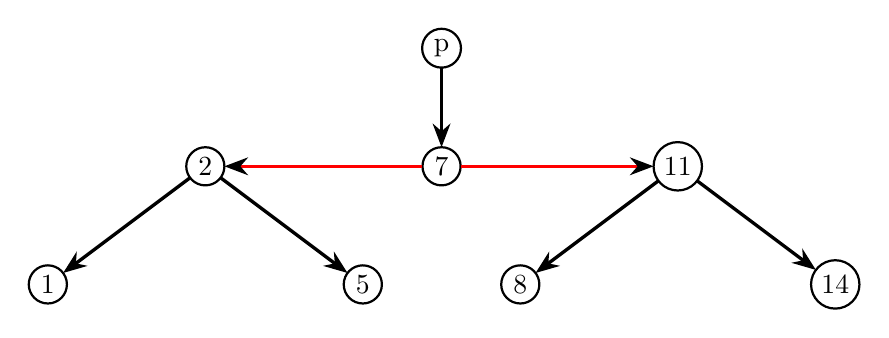
\begin{tikzpicture}
\begin{scope}[every node/.style={circle,inner sep=2pt,outer sep=0pt,thick,draw}]
    \node (p) at (0,1.5) {p};
    \node (7) at (0.00, 0.00) {7};
    \node (2) at (-3.00, 0.00) {2};
    \node (1) at (-5.00, -1.50) {1};
    \node (5) at (-1.00, -1.50) {5};
    \node (11) at (3.00, 0.00) {11};
    \node (8) at (1.00, -1.50) {8};
    \node (14) at (5.00, -1.50) {14};
\end{scope}
\begin{scope}[>={Stealth[black,length=3mm]},
              every node/.style={fill=white,circle},
              red_edge/.style={draw=red,very thick},
              black_edge/.style={draw=black,very thick}]
    \path [->] (p) edge [black_edge] (7);
    \path [->] (7) edge [red_edge] ({2});
    \path [->] (2) edge [black_edge] ({1});
    \path [->] (2) edge [black_edge] ({5});
    \path [->] (7) edge [red_edge] ({11});
    \path [->] (11) edge [black_edge] ({8});
    \path [->] (11) edge [black_edge] ({14});
\end{scope}
\end{tikzpicture}
\caption{Fix of \emph{Case 2.1} violation}
\label{fig:case_2_1_fix}
\end{figure}

Upon completion of this operation, node \encircle{7} (that is, the newly inserted node) becomes the new root, and no new
violation exists, since the root of the sub-tree under consideration is connected by a \emph{BLACK} link.

The resulting sub-tree is now balanced (Figure~\ref{fig:case_2_1_fix}).

\subsubsection{Case 2.2: Left child}

Consider now the second case, in which the node under consideration is the left child of its parent.
Suppose this node is node \encircle{2}, the left child of its parent, node \encircle{7}.
The uncle of node \encircle{2} is node \encircle{14}, which is a \emph{BLACK} node.

As before, the tree in Figure~\ref{fig:case_2_2_violation}. ``leans'' to the left, a condition that requires correction.

\begin{figure}[ht]
\centering
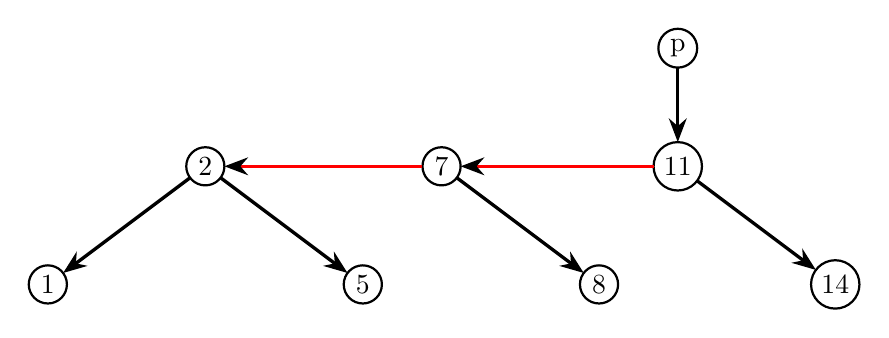
\begin{tikzpicture}
\begin{scope}[every node/.style={circle,inner sep=2pt,outer sep=0pt,thick,draw}]
    \node (p) at (3,1.5) {p};
    \node (7) at (0.00, 0.00) {7};
    \node (2) at (-3.00, 0.00) {2};
    \node (1) at (-5.00, -1.50) {1};
    \node (5) at (-1.00, -1.50) {5};
    \node (11) at (3.00, 0.00) {11};
    \node (8) at (2.00, -1.50) {8};
    \node (14) at (5.00, -1.50) {14};
\end{scope}
\begin{scope}[>={Stealth[black,length=3mm]},
              every node/.style={fill=white,circle},
              red_edge/.style={draw=red,very thick},
              black_edge/.style={draw=black,very thick}]
    \path [->] (p) edge [black_edge] (11);
    \path [->] (7) edge [red_edge] ({2});
    \path [->] (2) edge [black_edge] ({1});
    \path [->] (2) edge [black_edge] ({5});
    \path [->] (11) edge [red_edge] ({7});
    \path [->] (7) edge [black_edge] ({8});
    \path [->] (11) edge [black_edge] ({14});
\end{scope}
\end{tikzpicture}
\caption{Inserting a new node --- left child, uncle is \emph{BLACK}}
\label{fig:case_2_2_violation}
\end{figure}

The direction of the link $11 \rightarrow 7$ is reversed to $7 \rightarrow 11$.
Since node \encircle{7} becomes connected to node \encircle{11}, 
its right child is detached, and at the same time node \encircle{11} loses its left child.
In order to preserve the binary search tree property, node \encircle{11} is connected to node \encircle{8}.

Accordingly, this violation is corrected as follows:
\begin{enumerate}
    \item Delete the link $7 \rightarrow 8$
    \item Change the direction of link $11 \rightarrow 7$ to $7 \rightarrow 11$
    \item Create a \emph{BLACK} link $11 \rightarrow 8$
\end{enumerate}

\begin{figure}[ht]
\centering
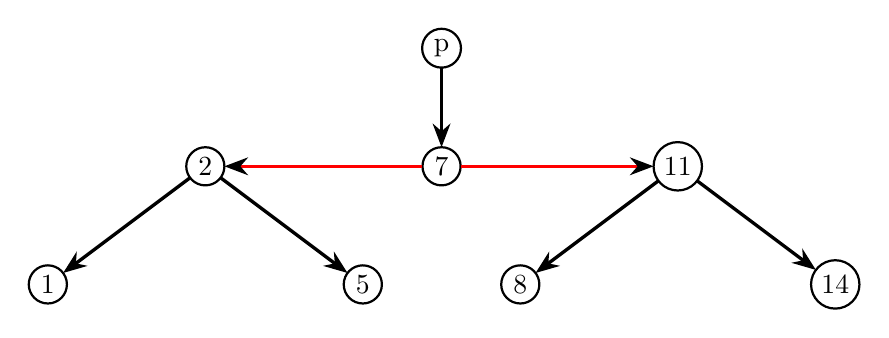
\begin{tikzpicture}
\begin{scope}[every node/.style={circle,inner sep=2pt,outer sep=0pt,thick,draw}]
    \node (p) at (0,1.5) {p};
    \node (7) at (0.00, 0.00) {7};
    \node (2) at (-3.00, 0.00) {2};
    \node (1) at (-5.00, -1.50) {1};
    \node (5) at (-1.00, -1.50) {5};
    \node (11) at (3.00, 0.00) {11};
    \node (8) at (1.00, -1.50) {8};
    \node (14) at (5.00, -1.50) {14};
\end{scope}
\begin{scope}[>={Stealth[black,length=3mm]},
              every node/.style={fill=white,circle},
              red_edge/.style={draw=red,very thick},
              black_edge/.style={draw=black,very thick}]
    \path [->] (p) edge [black_edge] (7);
    \path [->] (7) edge [red_edge] ({2});
    \path [->] (2) edge [black_edge] ({1});
    \path [->] (2) edge [black_edge] ({5});
    \path [->] (7) edge [red_edge] ({11});
    \path [->] (11) edge [black_edge] ({8});
    \path [->] (11) edge [black_edge] ({14});
\end{scope}
\end{tikzpicture}
\caption{Fix of \emph{Case 2.2} violation}
\label{fig:case_2_2_fix}
\end{figure}

Upon completion of this operation, all violations have been corrected, since a \emph{BLACK} link has been reached;
nothing further remains to be done.

Once again, the resulting sub-tree is now balanced (Figure~\ref{fig:case_2_2_fix}).

\section{Implementation}

In the source code listings of the remaining sections, a hypothetical language (pseudo-code) resembling
\texttt{C\#} or \texttt{Java} is used.

\subsection{Type RedBlackTree}

The type \texttt{RedBlackTree} contains at least these three functions:
\begin{lstlisting}[language=java]
public class RedBlackTree<K, V>
    where K: Comparable
{
    void Insert(K key, V value);
    bool Delete(K key);
    V? Search(K key);
}
\end{lstlisting}
The \texttt{Delete} function returns \emph{true} if the key was found in the tree and the corresponding node was
deleted, and \emph{false} otherwise. The \texttt{Search} function returns \texttt{NIL} when the \emph{key} is not found
in the tree.
\par

Optionally, \texttt{RedBlackTree} may provide a read-only \texttt{Size} property of type \texttt{Integer}, which returns
the number of keys in the tree.

\subsubsection{Comparing keys}

The \texttt{Comparable} interface contains a function that compares this key with another:
\begin{lstlisting}[language=java]
public interface Comparable<K>
{
    int CompareTo(K other);
}
\end{lstlisting}
If the implementation language does not support interfaces, a simple function comparing the two keys is sufficient,
for example:
\begin{lstlisting}[language=c]
int compare_to(K key1, K key2)
\end{lstlisting}
In either case, the function should return:
\begin{itemize}
    \item 0, if the two keys are equal.
    \item a value \textless0, if \emph{key1} is less than \emph{key2}.
    \item a value \textgreater0, if \emph{key1} is greater than \emph{key2}.
\end{itemize}

\subsection{Type Node}

Every node instance of a \emph{Red-Black} tree is of type \texttt{Node} that contains the following properties:
\begin{itemize}
    \item \emph{Key}, of a template type \texttt{K}.
    \item \emph{Value}, of a template type \texttt{V}.
    \item \emph{Color}, of a type \texttt{COLOR} an enumeration with values \texttt{RED} or \texttt{BLACK}.
    \item \emph{Left}, \emph{Right} of type \texttt{Node} reference.
\end{itemize}

\subsubsection{The parent node}

In many implementations the \texttt{Node} type contains a reference to its \emph{Parent} node.
Since this increases the memory consumption of the data structure and complicates the algorithms presented here,
a different approach is adopted: the ancestors of a node are determined by storing the path from the \emph{root} to the
position at which the new node is to be inserted, as the tree is traversed.
The \emph{parent}, \emph{grand-parent} and \emph{great-grand-parent} of a node are simply references within
the \texttt{Path} type, a specialized \emph{Stack} data structure initialized and populated in the \texttt{Insert}
function.

\subsubsection{Child direction}

Some algorithms make a decision based on whether a node is the left or the right child of its parent.
There is no need to store any additional information in each node (such as a property \texttt{bool IsLeftChild}),
since whether a node is the left or the right child of its parent can readily be determined by comparing it with the
\texttt{Left} or the \texttt{Right} property of the \emph{Parent},
provided that the \emph{Parent} is not \texttt{NIL}, that is, that the node is not the \emph{root}.

\subsubsection{Inserting the same key}

The implementation should handle the case of inserting a key-value pair whose key already exists in the tree. The
implementation may choose to:
\begin{itemize}
    \item skip the insertion.
    \item replace the existing value of the key with the new value.
    \item append the new value to a collection of values associated with the node for this key, typically only if the
    value is not already present in the collection. In this case each node stores a collection of values rather than a
    single value, and the \texttt{Search} function must return a collection of values when the key is found.
\end{itemize}

In the reference implementation, the \emph{value} of the node with the matching \emph{key} is replaced.

\subsubsection{The Sentinel node}

To simplify the handling of boundary conditions, rather than using \emph{NIL} references for leaf nodes or the root
node, a \emph{sentinel} node is used to represent a \emph{NIL} node:
\begin{lstlisting}[language=java]
public class RedBlackTree
{
    \\ ...
    const Node Nil = new Node { Color = Black };
}
\end{lstlisting}
The implementation may assign any suitable values to the \texttt{Key}, \texttt{Value},
\texttt{Left}, \texttt{Right} and \texttt{Parent} properties. Only the \texttt{Color} property is explicitly set to
\emph{BLACK}. In addition, the \texttt{Key} property of the \emph{Nil} node is set to the key used when searching, or
at the start of the insertion algorithm.
\par
It should be noted that not only all leaves but also the \emph{root} node are set to point to the \texttt{Nil} node.
This is consistent with the second rule of \emph{Red-Black} trees, which requires the \emph{root} node to be
\emph{BLACK}.
\par

\section{Searching}

The recursive implementation of the \texttt{Search} function is:
\begin{lstlisting}[language=java]
public V? Search(K key)
{
    // Set the key of the Nil node to the value of 
    // the key that we search. The value of the Nil
    // node is the default V value
    Nil.Key = key;

    return Search(Root, key);
}

private static V? Search(Node node, K key)
{
    var compare = key.CompareTo(node.Key);

    if (compare == 0) return node.Value;
    if (compare < 0) return Search(node.Left, key);
    return Search(node.Right, key);
}
\end{lstlisting}
Note that, because the sentinel is used in the private \texttt{Search} function,
there is no need to test whether a node is \emph{NIL}, thereby avoiding an additional condition in each recursive call.
Note further that the node found may be the \emph{Nil} node, in which case the value returned is the value of the
\emph{Nil} node, that is, \emph{NIL}.

The iterative version of the \texttt{Search} function is:
\begin{lstlisting}[language=java]
public V? IterativeSearch(K key)
{
    // Set the key of the Nil node to the value of 
    // the key that we search. The value of the Nil
    // node is the default V value
    Nil.Key = key;

    int compare;
    var node = Root;
    while ((compare = key.CompareTo(node.Key)) != 0)
    {
        if (compare < 0) node = node.Left;
        else node = node.Right;
    }

    return node.Value;
}
\end{lstlisting}

\section{Insert}

Using the techniques described in the previous sections, the insertion of a new key-value pair is straightforward.
First, the position at which the new node is to be placed is located. During this traversal, the \emph{path} is
initialized and populated, which subsequently enables the ancestors of the new node to be determined.

Any two consecutive \emph{RED} nodes violations that may occur are then corrected, moving upwards for as long as the
current node is \emph{RED}. At each iteration, the \emph{Propagation} and \emph{Rebalance} mechanisms described in the
previous sections are applied.

\begin{lstlisting}[language=java]
public void Insert(K key, V value)
{
    var x = Root;
    var y = Nil;
    int compare = 0;

    var path = new Path();
    path.Push(Nil);

    while (x != Nil)
    {
        path.Push(x);

        y = x;
        compare = key.CompareTo(x.Key);

        if (compare == 0)
        {
            x.Value = value;
            return;
        }

        if (compare < 0) x = x.Left;
        else x = x.Right;
    }

    var z = new Node<K, V>(key, value, Nil);

    if (y == Nil) Root = z;
    else if (compare < 0) y.Left = z;
    else y.Right = z;

    path.Push(z);
    InsertFixup(path);

    Size++;
}
\end{lstlisting}

\begin{lstlisting}[language=java]
private void InsertFixup(Path path)
{
    Node<K, V> p;

    while ((p = path.PeekParent()).IsRed)
    {
        var z = path.Peek();
        var gp = path.PeekGrandParent();

        if (p.IsLeftChildOf(gp))
        {
            var uncle = gp.Right;

            if (uncle.IsRed)
            {
                // Case 1
                p.Color = Color.Black;
                uncle.Color = Color.Black;
                gp.Color = Color.Red;
                path.Pop();
                path.Pop();
            }
            else
            {
                if (z.IsRightChildOf(p))
                {
                    // Case 2.1
                    if (Root == gp)
                    {
                        Root = z;
                    }
                    else
                    {
                        var gpp = 
                            path.PeekGreatGrandParent();
                        if (gp.IsLeftChildOf(gpp)) 
                            gpp.Left = z;
                        else
                            gpp.Right = z;
                    }

                    p.Right = z.Left;
                    gp.Left = z.Right;
                    z.Left = p;
                    p.Color = Color.Red;
                    z.Right = gp;
                    gp.Color = Color.Red;
                    z.Color = Color.Black;
                    break;
                }
                else
                {
                    // Case 2.2
                    if (Root == gp)
                    {
                        Root = p;
                    }
                    else
                    {
                        var gpp = 
                            path.PeekGreatGrandParent();
                        if (gp.IsLeftChildOf(gpp)) 
                            gpp.Left = p;
                        else
                            gpp.Right = p;
                    }

                    gp.Left = p.Right;
                    p.Right = gp;
                    gp.Color = Color.Red;
                    p.Color = Color.Black;
                    break;
                }
            }
        }
        else
        {
            var uncle = gp.Left;

            if (uncle.IsRed)
            {
                // Case 1
                p.Color = Color.Black;
                uncle.Color = Color.Black;
                gp.Color = Color.Red;
                path.Pop();
                path.Pop();
            }
            else
            {
                if (z.IsLeftChildOf(p))
                {
                    // Case 2.1
                    if (Root == gp)
                    {
                        Root = z;
                    }
                    else
                    {
                        var gpp = 
                            path.PeekGreatGrandParent();
                        if (gp.IsLeftChildOf(gpp))
                            gpp.Left = z;
                        else
                            gpp.Right = z;
                    }

                    p.Left = z.Right;
                    gp.Right = z.Left;
                    z.Right = p;
                    p.Color = Color.Red;
                    z.Left = gp;
                    gp.Color = Color.Red;
                    z.Color = Color.Black;
                    break;
                }
                else
                {
                    // Case 2.2
                    if (Root == gp)
                    {
                        Root = p;
                    }
                    else
                    {
                        var gpp =
                            path.PeekGreatGrandParent();
                        if (gp.IsLeftChildOf(gpp))
                            gpp.Left = p;
                        else
                            gpp.Right = p;
                    }

                    gp.Right = p.Left;
                    p.Left = gp;
                    gp.Color = Color.Red;
                    p.Color = Color.Black;
                    break;
                }
            }
        }
    }

    Root!.Color = Color.Black;
}
\end{lstlisting}

\section{Conclusion}

This paper has sought to explain the mechanisms underlying \emph{Red-Black} trees in a visual manner.
It is argued that the true meaning of the rotations used in \emph{Red-Black} trees is harder to grasp, and that the
\emph{Propagation} and \emph{Rebalance} mechanisms are more readily assimilated in a visual manner by a reader
encountering \emph{Red-Black} trees for the first time.

\printbibliography

\end{document}
